\subsection{Hole detection via RGB-D camera within the RoboCup Rescue competition}

Context: Voluntary work at PANDORA Robotics group, Aristotle University of
Thessaloniki, Thessaloniki, Greece.\\\\
\url{http://pandora.ee.auth.gr/}\\
\url{https://github.com/pandora-auth-ros-pkg}\\

Within the context of the RoboCup Rescue competition, robotic rescuers have to
be able to locate victims in closed spaces (simulating what is to happen during
emergency situations) and therefore have to first detect the ``holes" in walls
behind which the victims are located. The unmanned ground vehicle PANDORA
uses a RGB and a Depth camera for such purposes. Each of the images of the two
cameras undergo independent analyses so as to make locating the precise
outline of holes more probable. Figure \ref{fig:holes} shows the outcome of
such analyses after cross-referencing RGB-derived holes to Depth-derived holes
and vice versa, and after further processing. In terms of time, the resulting
ROS package took around seven months to build; in terms of size it is comprised
of around 8K lines of code and 4K lines of comments.

%\begin{figure}[H]\centering
  %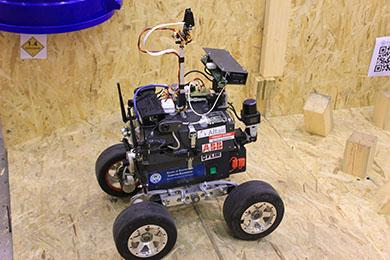
\includegraphics[scale=1]{images/pandora_robot.jpg}
  %\caption{}
  %\label{fig:pandora_robot}
%\end{figure}

\begin{figure}[H]\centering
  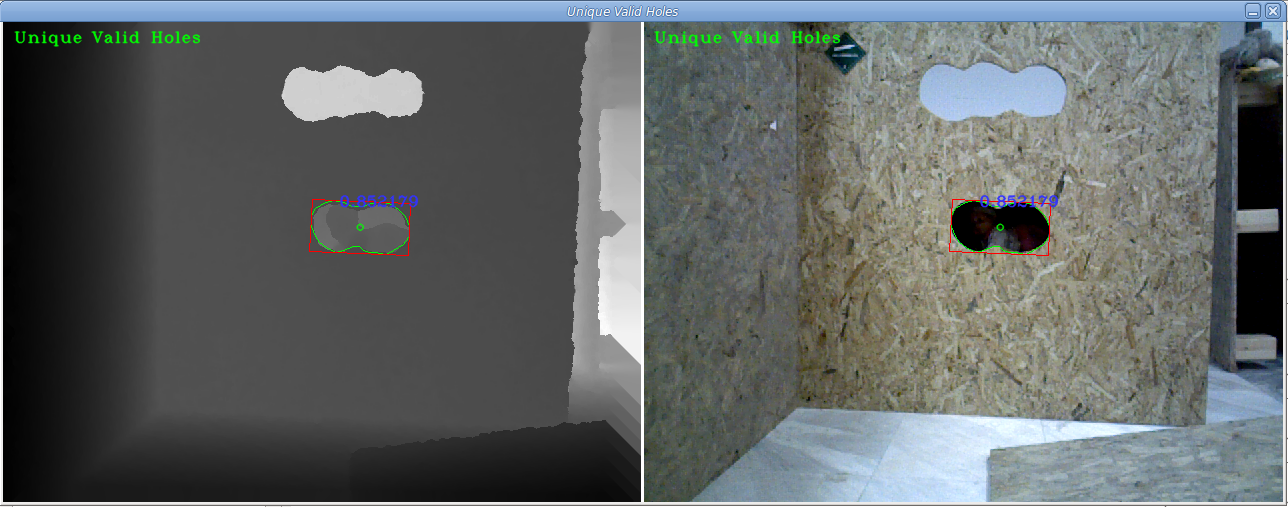
\includegraphics[scale=0.35]{images/unique_holes.png}
  \caption{Although the wall has two holes, only the one closer to the ground
    is valid: the hole above it is through-and-through and therefore cannot
    contain possible victims.}
  \label{fig:holes}
\end{figure}


Resources / tools involved: C++, ROS, git(hub)
